\documentclass{article}

% Símbolos
\usepackage{recycle}
\usepackage{amsfonts}

% Figuras
\usepackage{graphicx}

% Gráficas
\usepackage{tikz}

% Estilo Tikz
\tikzstyle{edge}=[shorten <=2pt, shorten >=2pt,
                  >=stealth, line width=1.1pt]
\tikzstyle{vertex}=[circle, fill=white, draw,
                    minimum size=5pt,
                    inner sep=0pt, outer sep=0pt]

% Márgenes
\addtolength{\voffset}{-1cm}
\addtolength{\hoffset}{-1.5cm}
\addtolength{\textwidth}{3cm}
\addtolength{\textheight}{2cm}

% Encabezados y Pies de Página
\usepackage{fancyhdr}
% Información del Encabezado
\lhead{Teor\'ia de Gr\'aficas II 2021-2 \\
       Tarea 1}
\rhead{Profesor: C\'esar Hern\'andez Cruz \\
       Ayudante: Daniel Garc\'ia Argueta}
% Información del Pie de Página
\rfoot{\recycle}
\cfoot{\vspace{-0.8cm}?`Realmente necesitas imprimir esta hoja?}
\lfoot{\recycle}
\pagenumbering{gobble}
\footskip = 50pt
% Línea del encabezado
\renewcommand\headrulewidth{1.5pt}
%%%%%%%%%%%%%%%%%%%%%%%%%%%%%%%%%%%%%%%%%%%%%%%%%%%%%%%%%%%%%
%%%%%%%%%%%%%%%%%%%%%%%%%%%%%%%%%%%%%%%%%%%%%%%%%%%%%%%%%%%%%
%%%%%%%%%%          Gráfica en encabezado          %%%%%%%%%%
%%%%%%%%%%%%%%%%%%%%%%%%%%%%%%%%%%%%%%%%%%%%%%%%%%%%%%%%%%%%%
%%%%%%%%%%%%%%%%%%%%%%%%%%%%%%%%%%%%%%%%%%%%%%%%%%%%%%%%%%%%%
\makeatletter
\def\headrule{{\if@fancyplain\let\headrulewidth\plainheadrulewidth\fi
\hrule\@height\headrulewidth\@width\headwidth
\vspace{0.1cm}
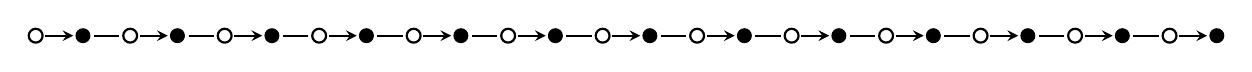
\begin{tikzpicture}
  \begin{scope}[scale=0.6]
   \foreach \x in {0,2,...,24} {
      \node [circle,draw,thick,inner sep=0,minimum size=5pt] (\x) at (\x,0){};
   }
   \foreach \x in {1,3,...,25} {
      \node [circle,draw,fill=black,inner sep=0,minimum size=5pt] (\x) at (\x,0){};
   }
   \foreach \x/\y in {0,2,...,24} {
     \pgfmathsetmacro\result{\x + 1}
     \draw [->,>=stealth,shorten <=3.5pt, shorten >=3.5pt,line width=0.7pt] (\x,0) to (\result,0);
   }
   \foreach \x/\y in {1,3,...,23} {
     \pgfmathsetmacro\result{\x + 1}
     \draw [>=stealth,shorten <=4pt, shorten >=4pt,line width=0.7pt] (\x,0) to (\result,0);
   }
   % \node [inner sep=0,minimum size=5pt] (25.5) at (25.5,-0.05){$\cdots$};
  \end{scope}
\end{tikzpicture}
\vskip-\headrulewidth
\vskip-1.5pt}}
\makeatother
%%%%%%%%%%%%%%%%%%%%%%%%%%%%%%%%%%%%%%%%%%%%%%%%%%%%%%%%%%%%%
%%%%%%%%%%%%%%%%%%%%%%%%%%%%%%%%%%%%%%%%%%%%%%%%%%%%%%%%%%%%%
%%%%%%%%%%%%%%%%%%%%%%%%%%%%%%%%%%%%%%%%%%%%%%%%%%%%%%%%%%%%%
%%%%%%%%%%%%%%%%%%%%%%%%%%%%%%%%%%%%%%%%%%%%%%%%%%%%%%%%%%%%%
%%%%%%%%%%%%%%%%%%%%%%%%%%%%%%%%%%%%%%%%%%%%%%%%%%%%%%%%%%%%%

% Estilo
\pagestyle{fancyplain}

% Macros
\newcommand{\set}[1]{\left\{ #1 \right\}}


\begin{document}

\begin{enumerate}
  \item Demuestre que si $D$ es una digr\'afica, entonces su
    condensaci\'on $D^\ast$ es ac\'iclica.

  \item Demuestre que si $D$ es una digr\'afica ac\'iclica, entonces
    tiene un \'unico n\'ucleo.   Adem\'as, a partir de su demostraci\'on
    obtenga un algoritmo para encontrar un n\'ucleo en una digr\'afica
    ac\'iclica.   ?`Qu\'e complejidad tiene su algoritmo?

  \item Demuestre que cualquier digr\'afica con al menos dos n\'ucleos
    contiene un ciclo par.

  \item Sea $D$ una digr\'afica fuertemente conexa y sea $k > 1$ un entero.
    Demuestre que si todos los ciclos de $D$ tienen longitud congruente a
    $0$ m\'odulo $k$, entonces $V$ admite una partici\'on $V = (V_0, \dots,
    V_{k-1})$ de tal forma que si $(u,v) \in A$, entonces existe $i \in
    \{ 0, \dots, k-1 \}$ tal que $u \in V_i$ y $v \in V_{i+1}$ donde los
    sub\'indices se toman m\'odulo $k$.

  \item Sea $D$ una digr\'afica infinita.  Demuestre que son equivalentes:
    \begin{enumerate}
      \item $D$ es n\'ucleo perfecta.

      \item Toda subdigr\'afica inducida de $D$ contiene un semin\'ucleo no
        vac\'io.
    \end{enumerate}
    (Sugerencia: Lema de Zorn.)

  \item Para cada entero $k \ge 2$ exhiba una gr\'afica bipartita cuyo
    n\'umero crom\'atico por listas sea al menos $k$.

  \item Demuestre que la digr\'afica de la Figura \ref{fig:choose} tiene
    n\'umero crom\'atico por listas igual a $3$.
    \label{eje:choose}
    \begin{figure}[ht!]
    \centering
    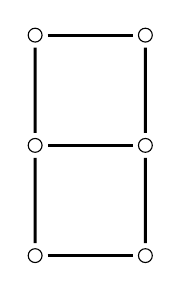
\begin{tikzpicture}
    \begin{scope}[scale=0.7]
      \node (a) at (-1,2)  [vertex]{};
      \node (b) at (-1,0)  [vertex]{};
      \node (c) at (-1,-2) [vertex]{};
      \node (x) at (1,2)   [vertex]{};
      \node (y) at (1,0)   [vertex]{};
      \node (z) at (1,-2)  [vertex]{};

      \foreach \u/\v in {a/b,a/x,y/x,y/b,y/z,c/b,c/z}
        \draw [edge] (\u) to (\v);
    \end{scope}
    \end{tikzpicture}
    \caption{Gr\'afica para el Ejercicio \ref{eje:choose}.}
    \label{fig:choose}
    \end{figure}
\end{enumerate}
\end{document}
